\documentclass[a4paper,12pt]{article}
\usepackage[a4paper,margin=1in,footskip=0.25in]{geometry}
\usepackage[utf8]{inputenc}

% science
\usepackage{amsmath}
\usepackage{array}
\usepackage{siunitx}

% layout
\usepackage{float}
\usepackage{parskip}
\usepackage{graphicx}
\usepackage{longtable}
\usepackage{hyperref}

\usepackage{caption}
\usepackage{subcaption}
\usepackage{wrapfig}


% referencing
\usepackage[style=apa]{biblatex}
\addbibresource{azero.bib}
\usepackage{hyperref}


% figures labelings
\usepackage{chngcntr}
\counterwithin{figure}{section}

\renewcommand{\arraystretch}{1.7}
\newcolumntype{P}[1]{>{\raggedright\arraybackslash}p{#1}}
\newcommand{\tptt}{$\times\,$}

% uncertainty
\newcommand{\absun}{\Delta \text{unc}\,}
\newcommand{\relun}{\% \text{unc}\,}

\title{Empirically finding the value of absolute zero using the ideal gas law}
\author{Terry Qi}

\begin{document}

\maketitle

\section{Design}
\subsection{Introduction}
% When we were introduced to the unit Kelvin in chemistry, I was initially confused by the need of a

During a trip for the purpose of completing my duke of edinburgh, when we have reached the hilltop and was resting for the descent, my supervisor --- which happened to be a physics teacher, told us that because at higher attitude water boils easier, thus at a lower maximum temperature, hikers cannot rely on the boiling of the water to purify it. For I am a frequent hiker, I first pondered, then decided to dig into the reasoning of this phenomenon. Initially I thought to conduct the experiment of the effects of altitude against the boiling point of water, but weather conditions quickly brushed away that idea. Through my research it seems that it is the decrease in atmospheric pressure that causes decrease the temperature needed for boiling, therefore I decided to investigate the relationship between temperature and pressure, and accidentally realizing its connection to a fundamental quantity when I extrapolate the recession line. While I've been told in class that the temperature of absolute zero is not physically reachable and is only useful in calculations, I now have a simple yet powerful procedure that calculates this variable. This investigation aims to empirically find the value of absolute zero using the temperature and pressure relationships.


\subsection{Research Question}
\begin{quote}
    What is the relationship between the pressure of room air mixture against its temperature under constant volume and quantity?
\end{quote}

\subsection{Background}
% talk about gases and the ideal gas law
There exists a wide range of chemical reactions that includes a variety of gases as reactants or products. For the sake of stoichiometric analysis, it is heavily desirable to be able to measure the number of moles of a gas. To ease the calculations involved with millions of individual gas particle at the microscopic level, the field of kinetic theory of matter created a model of the ideal gas with optimistic attributes attached that still resembles real gases in the world.

The five assumptions of an ideal gas are that: (1) the gas molecule collisions are elastic, (2) the volume of the particles are negligible, (3) there exists no intermolecular forces between the particles, (4) the particles of a gas obey Newtonian motion and move with a range of speed and direction \parencite{gas_law}. These assumptions will be crucial in designing my experiment.

With the help of numerous scientists over the span of 200 years, the model of the ideal gas law can be summarized in figure \ref{fig:igl}.

\begin{figure}[H]
    \[
    PV = nRT
    \]
    \caption{The Ideal Gas Law}
    \label{fig:igl}
\end{figure}

The law contains the relationships between the four gaseous state quantities, each in their respective standard units: $P$ for Pressure, $V$ for Volume, $n$ for number of moles, and $T$ for temperature. We are interested in strictly the relationship between temperature and pressure, thus extracting from the law, we arrive to the relationship in figure \ref{fig:pt}, where $c$ is the proportionality constant. This relation is also initially discovered by Joseph Louis Gay-Lussac.

\begin{figure}[H]
    \[
    P = cT
    \]
    \caption{Pressure and Temperature relationship}
    \label{fig:pt}
\end{figure}

The relationship showcases that as temperature of an ideal gas increases, its pressure also increases. This is because pressure measures the average force per area of the moving particles in the gas elastically colliding with the walls of the container. For temperature is a measure of the average kinetic energy of the particles, its increase is a description of faster moving particles, causing an average larger force on the gas container \parencite{pearson}.

% For there is a linear relationship between pressure and temperature, in the case of an ideal gas, I should measure a linear trend when graphing the gas pressure against its temperature, with an intercept of zero when the units are standard (Pascals and Kelvin).% 


\begin{wrapfigure}{r}{0.5\textwidth}
    \centering
    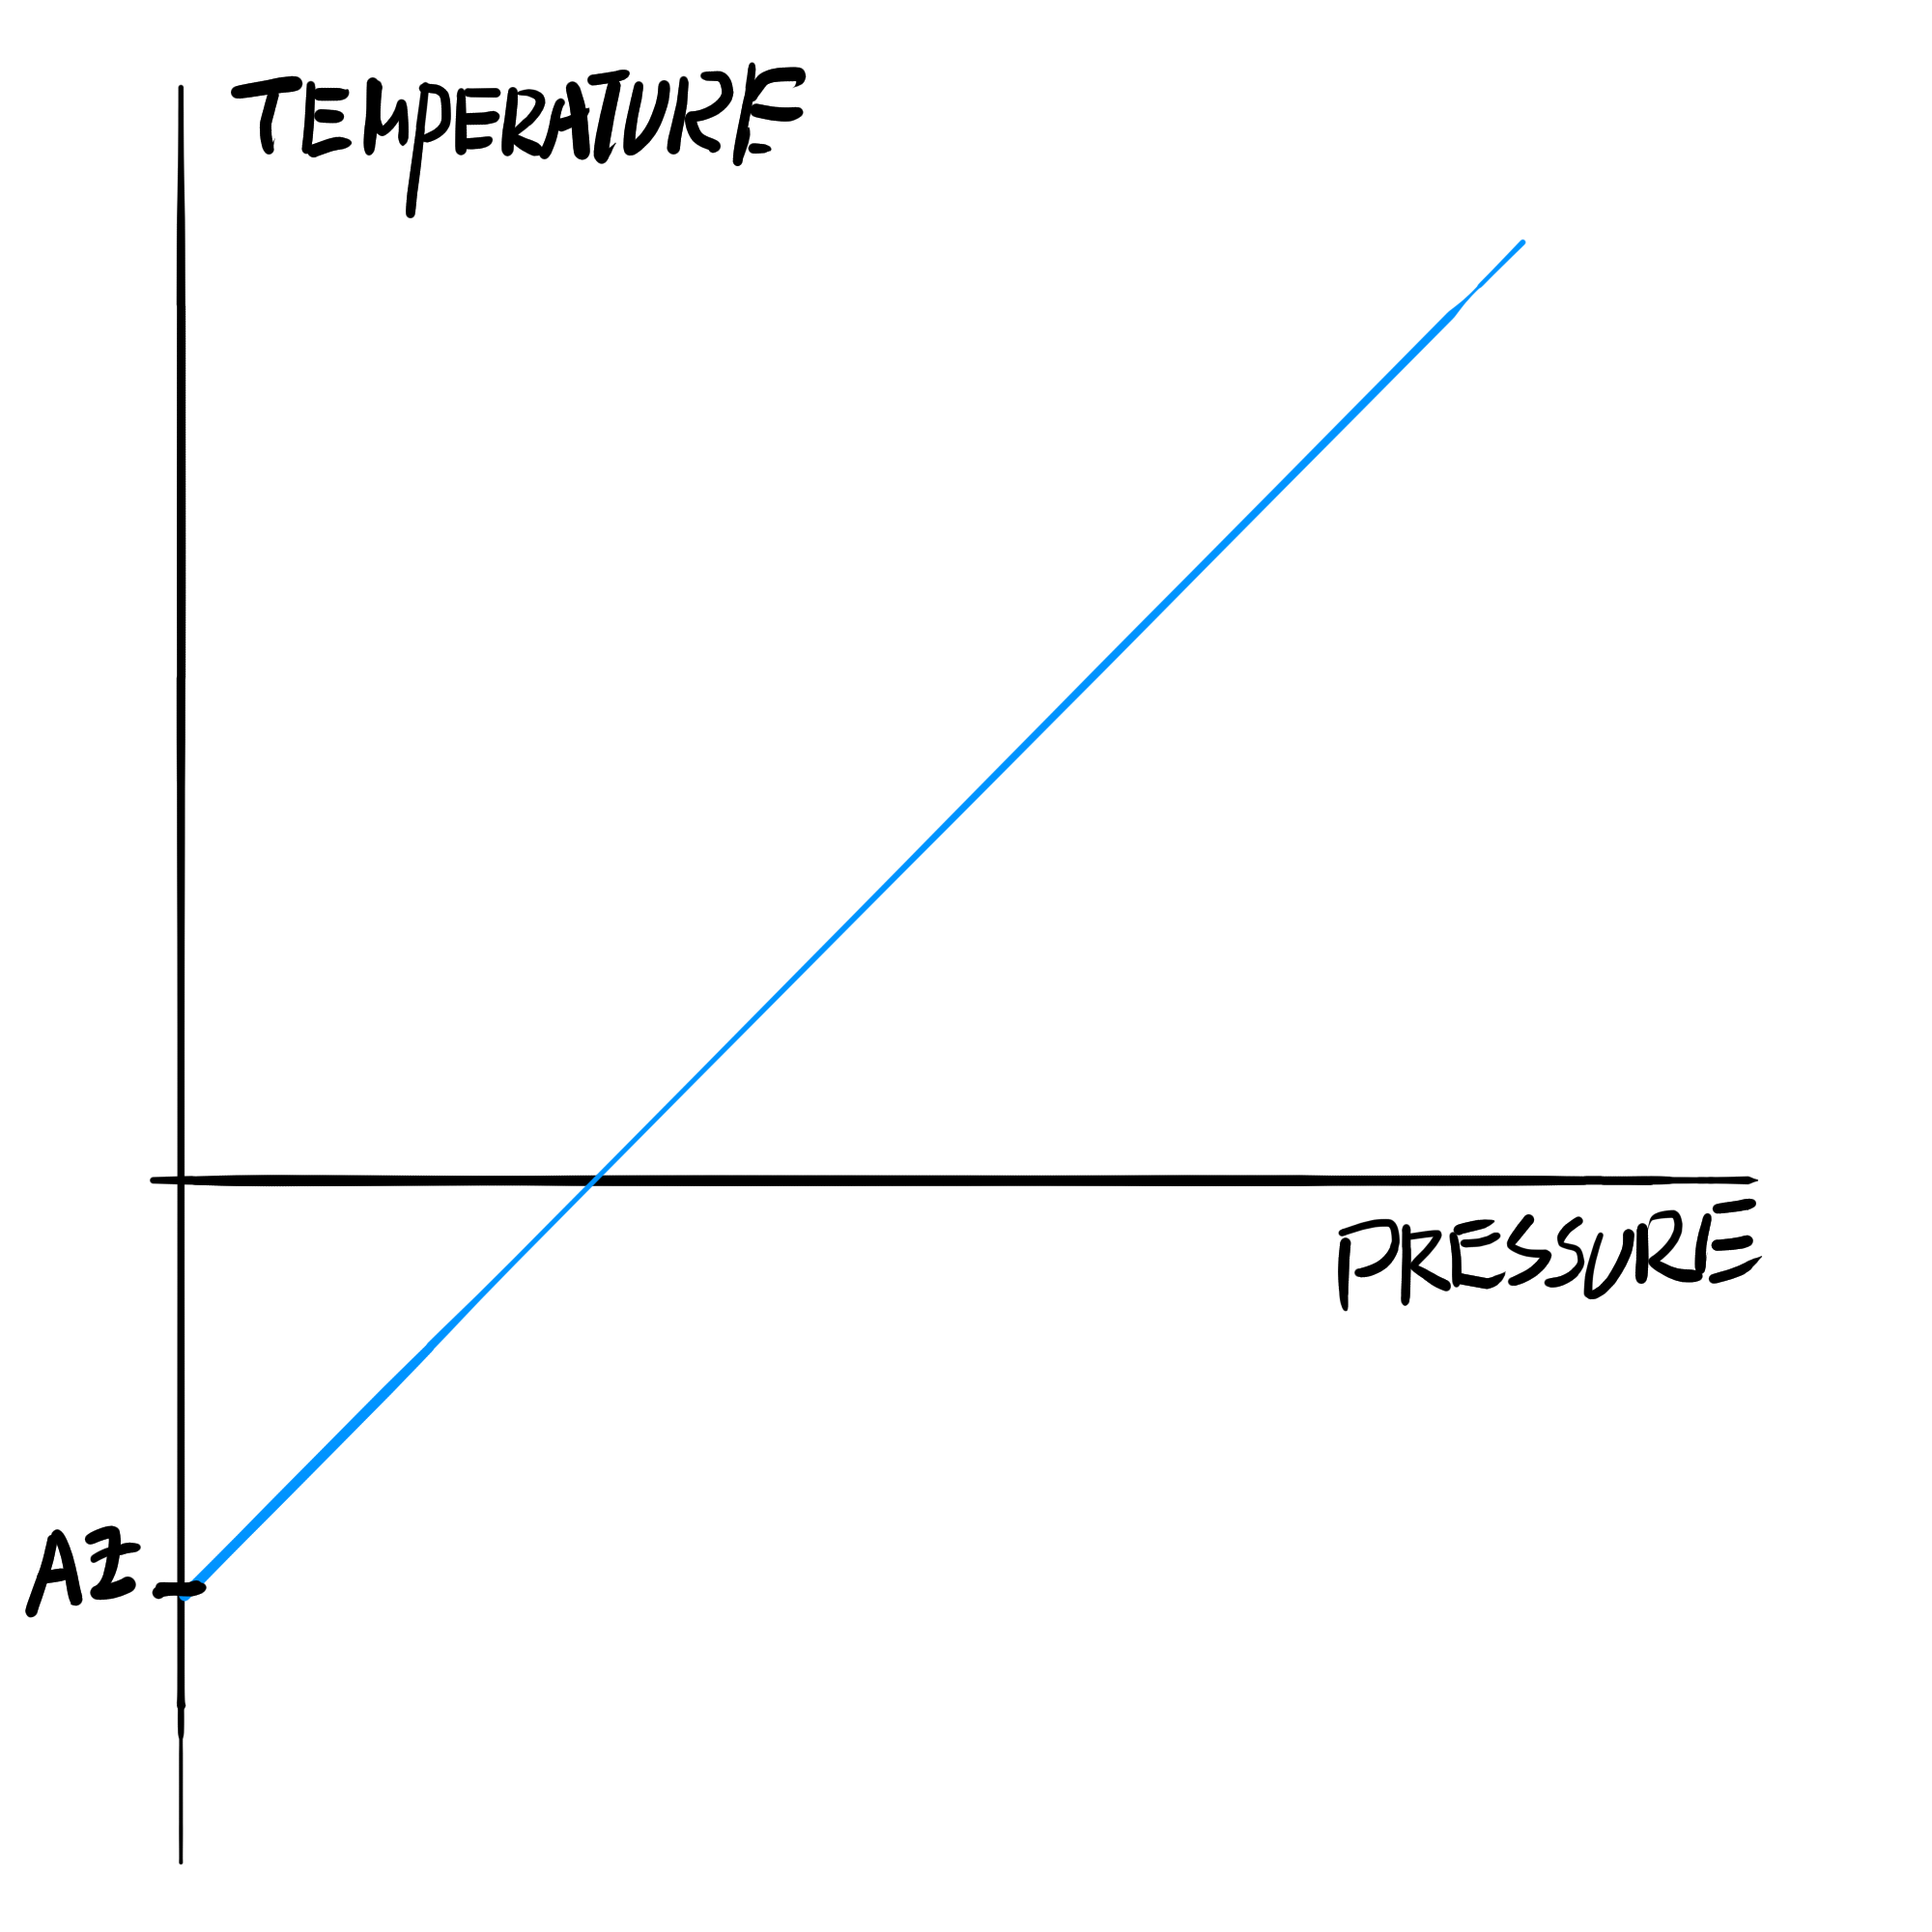
\includegraphics[width=0.4\textwidth]{assets/az.png}
    \caption{Transposed T vs. P graph}
    \label{fig:az}
\end{wrapfigure}

% its connection to the idea of absolute zero
However, by transposing the two axis (so that it is a Temperature against Pressure graph), extrapolating the linear relationship:
\[
    T = \frac{1}{c}P,
\]
can display an incredible result. The absolute zero is a theoretical measurement of temperature that sets the lower bound of the temperature scale. At the temperature, the movements of the gas particles are precisely zero, therefore the gas has zero outwards pressure. Therefore the y-intercept (AZ) of the regression line (figure \ref{fig:az}), should be zero when using an standard unit such as Kelvin, and would measure the value of absolute zero in Celsius when the temperature unit is in Celsius.


% https://en.wikipedia.org/wiki/Barometric_formula?oldformat=true
% Additionally, the proportionality constant $k$ can be used to determine the boiling point of water at a range of attitudes. A substance boils when the average kinetic energy of the particles exceeds average kinetic energy of the surrounding air. Macroscopically, this occurs when the pressure of the liquid is higher than the atmospheric pressure. The barometric function $P(h)$ is a mapping between heights and the atmospheric pressure, therefore we can deduce the boiling point


% how I would measure it
% potential source of errors
To test the theory, I have decided to use a pressure probe dipped in water above a bunsen burner, where temperature of the water is the independent variable and pressure of the air mixture is the dependent variable. The chosen range of temperature is from $20\si{\celsius}$ to $100\si{\celsius}$, for it ensures the widest possible range of temperatures of water (room temperature to boiling point) for regression.

For the gas is transparent to my eye, the gas mixture tested is likely to have minimal size. In combination with the perceived large volume of the container, the gas can be modeled with the ideal gas law. Therefore I hypothesize a positive correlation between the temperature and the pressure of the mixture, approximating a linear graph to that of figure \ref{fig:az}.

\subsection{Variables}
\paragraph{Independent Variable}
The temperature of the air mixture in unit Celsius

\paragraph{Dependent Variable}
The pressure of the air mixture in unit Pascal

\subsection{Control Variables}

% table here
\begin{longtable}{P{0.2\textwidth}|P{0.35\textwidth}|P{0.35\textwidth}}
Controls & Reason & How\\\hline

Volume of water in beaker & The quantity of water determines the submersion depth of the pressure probe, changing the area in contact with water, causing discrepancy in water and air mixture temperature, systematically lower pressure measurements & Use a constant, large enough volume (200ml) of water for each trials. The water should submersion the spherical bulb up to the stem, but not too much as to cause overflow \\

Interval between measurements & High pressure probe inaccuracy means changing temperature may not reflect in change in pressure, increasing random errors when measurements are taken too swiftly & Use a timer to take measurements every 30 seconds when heating, and every 1 minute when cooling, as to ensure meaningful pressure changes during the interval \\

Placement of sensors & Contact between the sensors and the beaker will cause systematic error in the difference in gas mixture and water temperature & Using clamps to suspend the thermometer and gas pressure probe within the water, avoid direct contact between any sensor \\

Environmental atmospheric pressure & Changes in the surrounding atmospheric pressure can systemically increase the pressure measurements & Conduct the experiment at the same location for each trial, ideally all within a short time span of a week
\\
Method of measurements & Non-direct viewing of the pressure probe will cause parallax error in pressure measurements. Guessing dim thermometer readings can create random errors in the IV & View the pressure probe upright and direct, prepare a backup thermometer to switch out if the current one is dim or hard to read \\
\end{longtable}

\subsection{Materials}

\begin{itemize}
    \item gas pressure measurement probe ($\pm 0.25\si{psi}$) (figure \ref{fig:probe})
    \item 500ml glass beaker with volume markings
    \item 2 $\times$ digital thermometer ($\pm 0.1\si{C}$)
    \item 2 $\times$ retort stands
    \item phone or a stopwatch as a timer ($\pm 1\si{s}$)
    \item bunsen burner, tripod, and heating mat
    \item lighter
\end{itemize}

\subsection{Method}


\begin{enumerate}
    \item Setup the experiment as shown as in figure \ref{fig:setup}, using two retort stands \& clamps, the bunsen burner setup, and an empty 500ml glass beaker.
    \item Lift the two clamps holding the gas pressure measurement probe. Fill the glass beaker with tap water, stop at approximately 200ml. Carefully reinsert the two sensors into the water.
    \item Wait for 1 minute for the sensors to stabilize. Then light the bunsen burner, start the timer, and record the first reading of temperature and pressure.
    \item Record the temperature and pressure every 30 seconds using the timer, stop the bunsen burner when the temperature reads above 100$\si{\celsius}$. Carefully change the thermometer if the displays become hard to read.
    \item Record the temperature and pressure every minute using the timer, stop recording when the temperature reads below around 65$\si{\celsius}$. Carefully remove the beaker and clean it with fresh water.
    \item Repeat step step 2-5 for a total of 5 times, noting the pressure and temperature data each time.
\end{enumerate}

\subsection{Diagrams}


\begin{figure}[H]
    \centering
    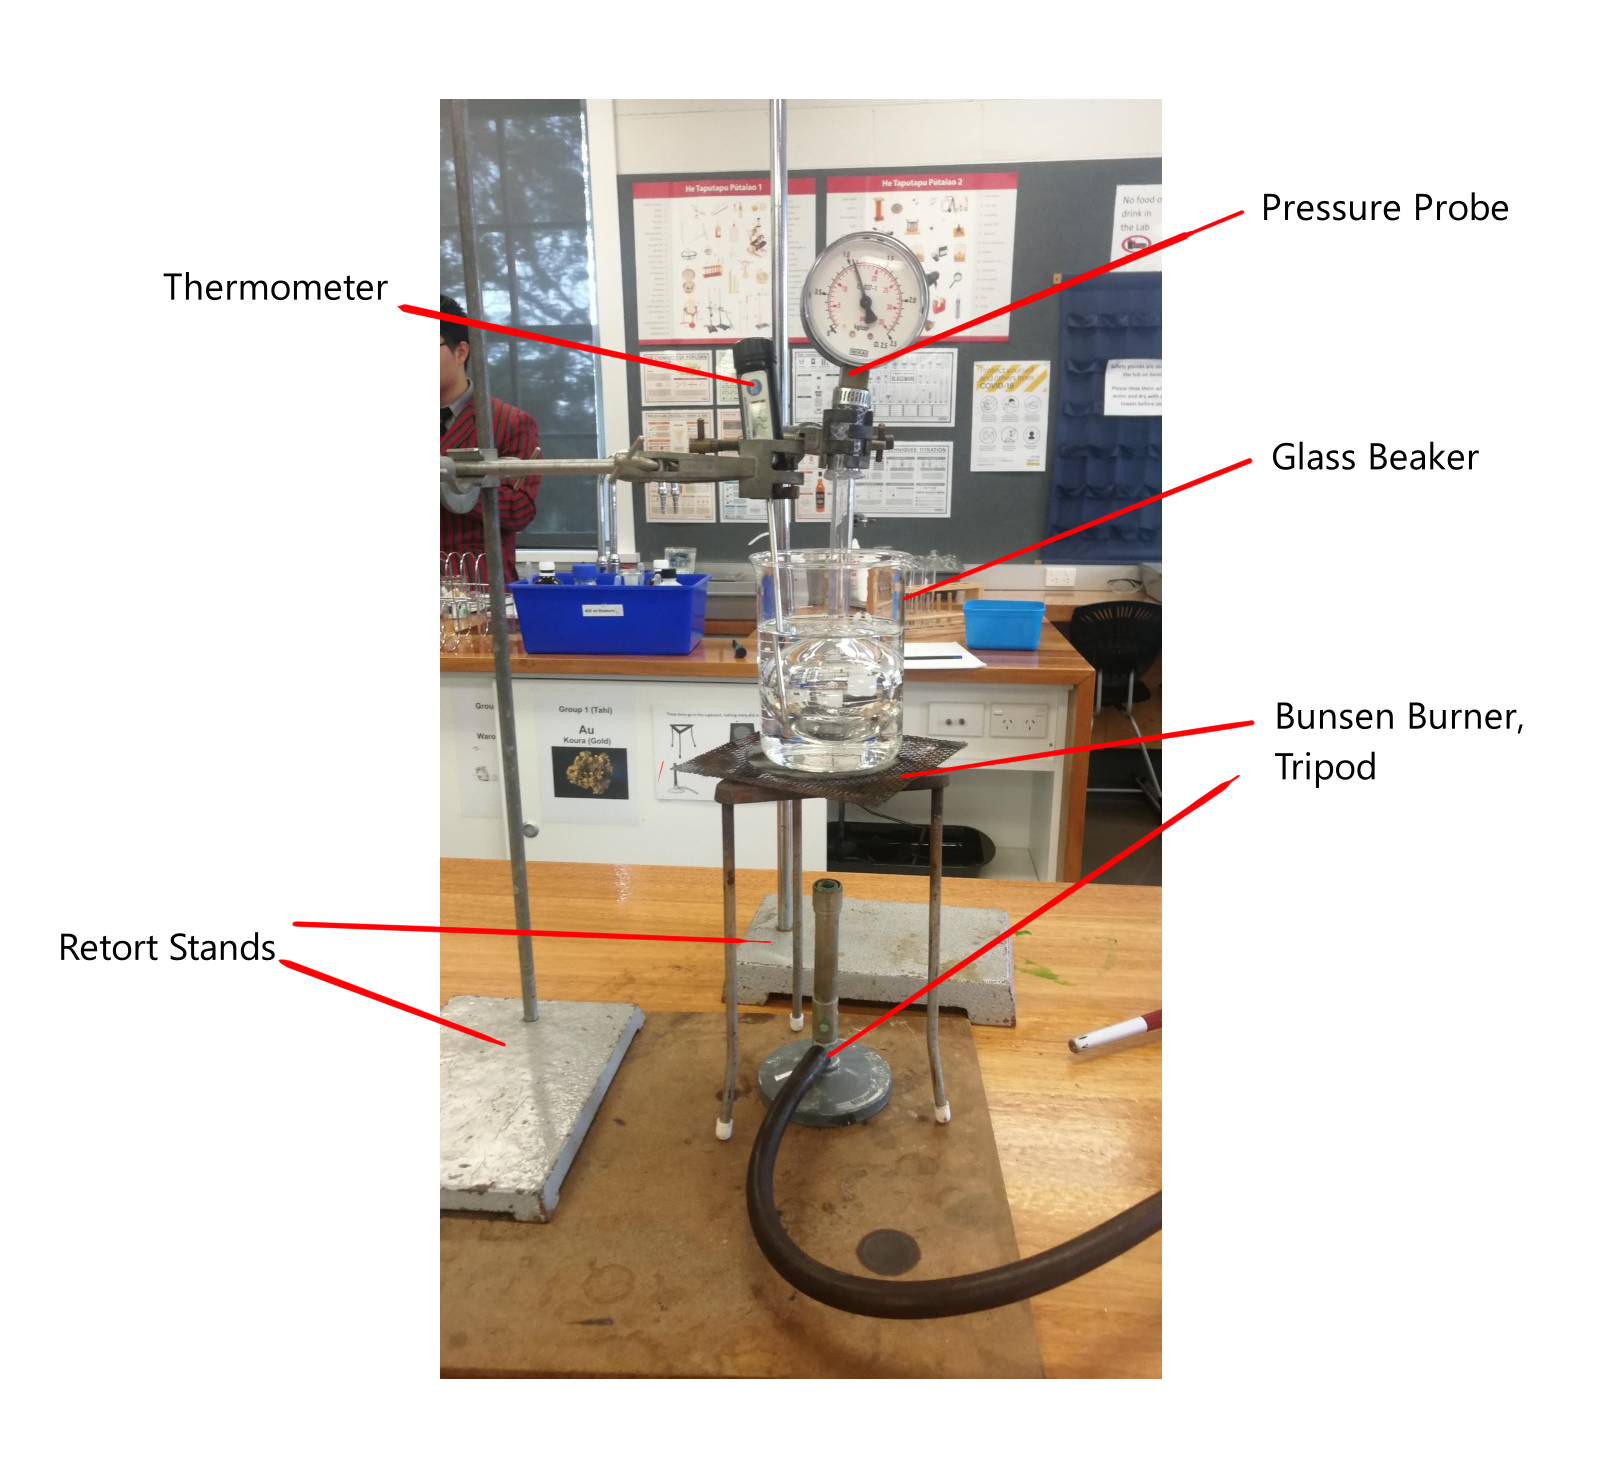
\includegraphics[width=\textwidth]{assets/setuplabelled.png}
    \captionof{figure}{An image of the experiment setup}
    \label{fig:setup}
\end{figure}

\begin{figure}[H]
    \centering
    \begin{minipage}{.4\textwidth}
        \centering
        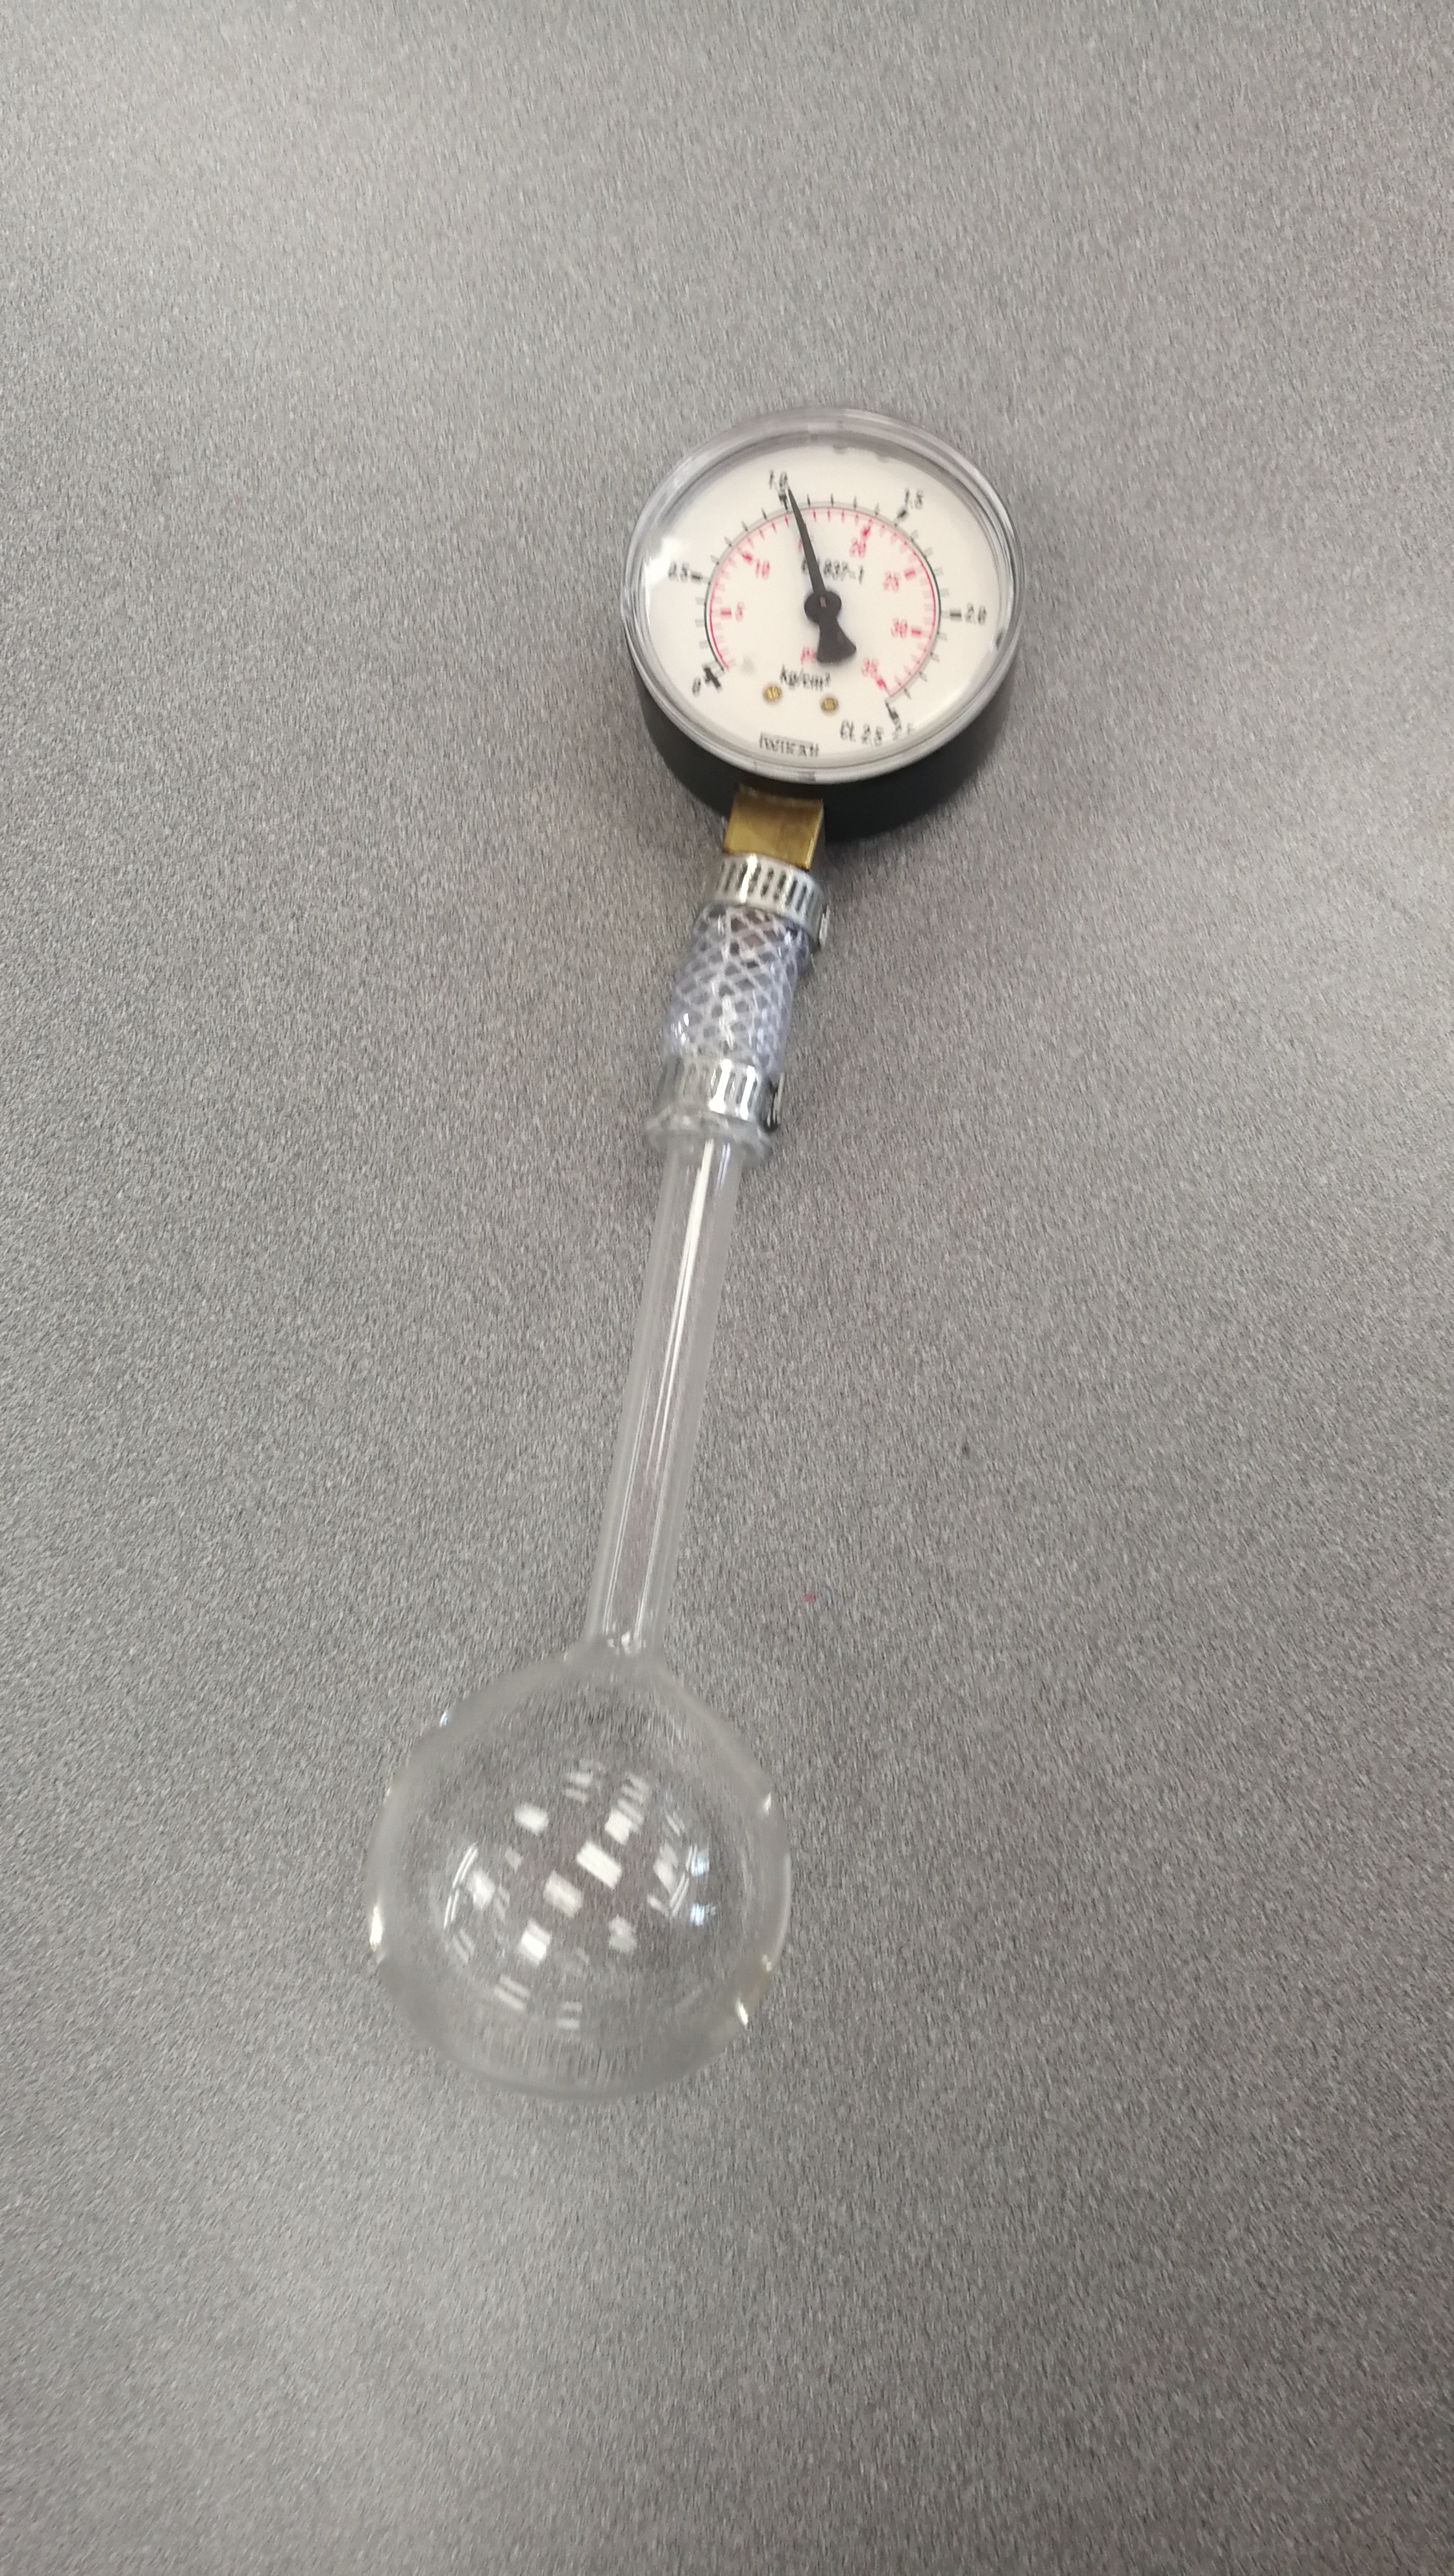
\includegraphics[scale=0.06]{assets/probe.jpg}
        \captionof{figure}{The gas pressure probe}
        \label{fig:probe}
    \end{minipage}%
    \begin{minipage}{.6\textwidth}
        \centering
        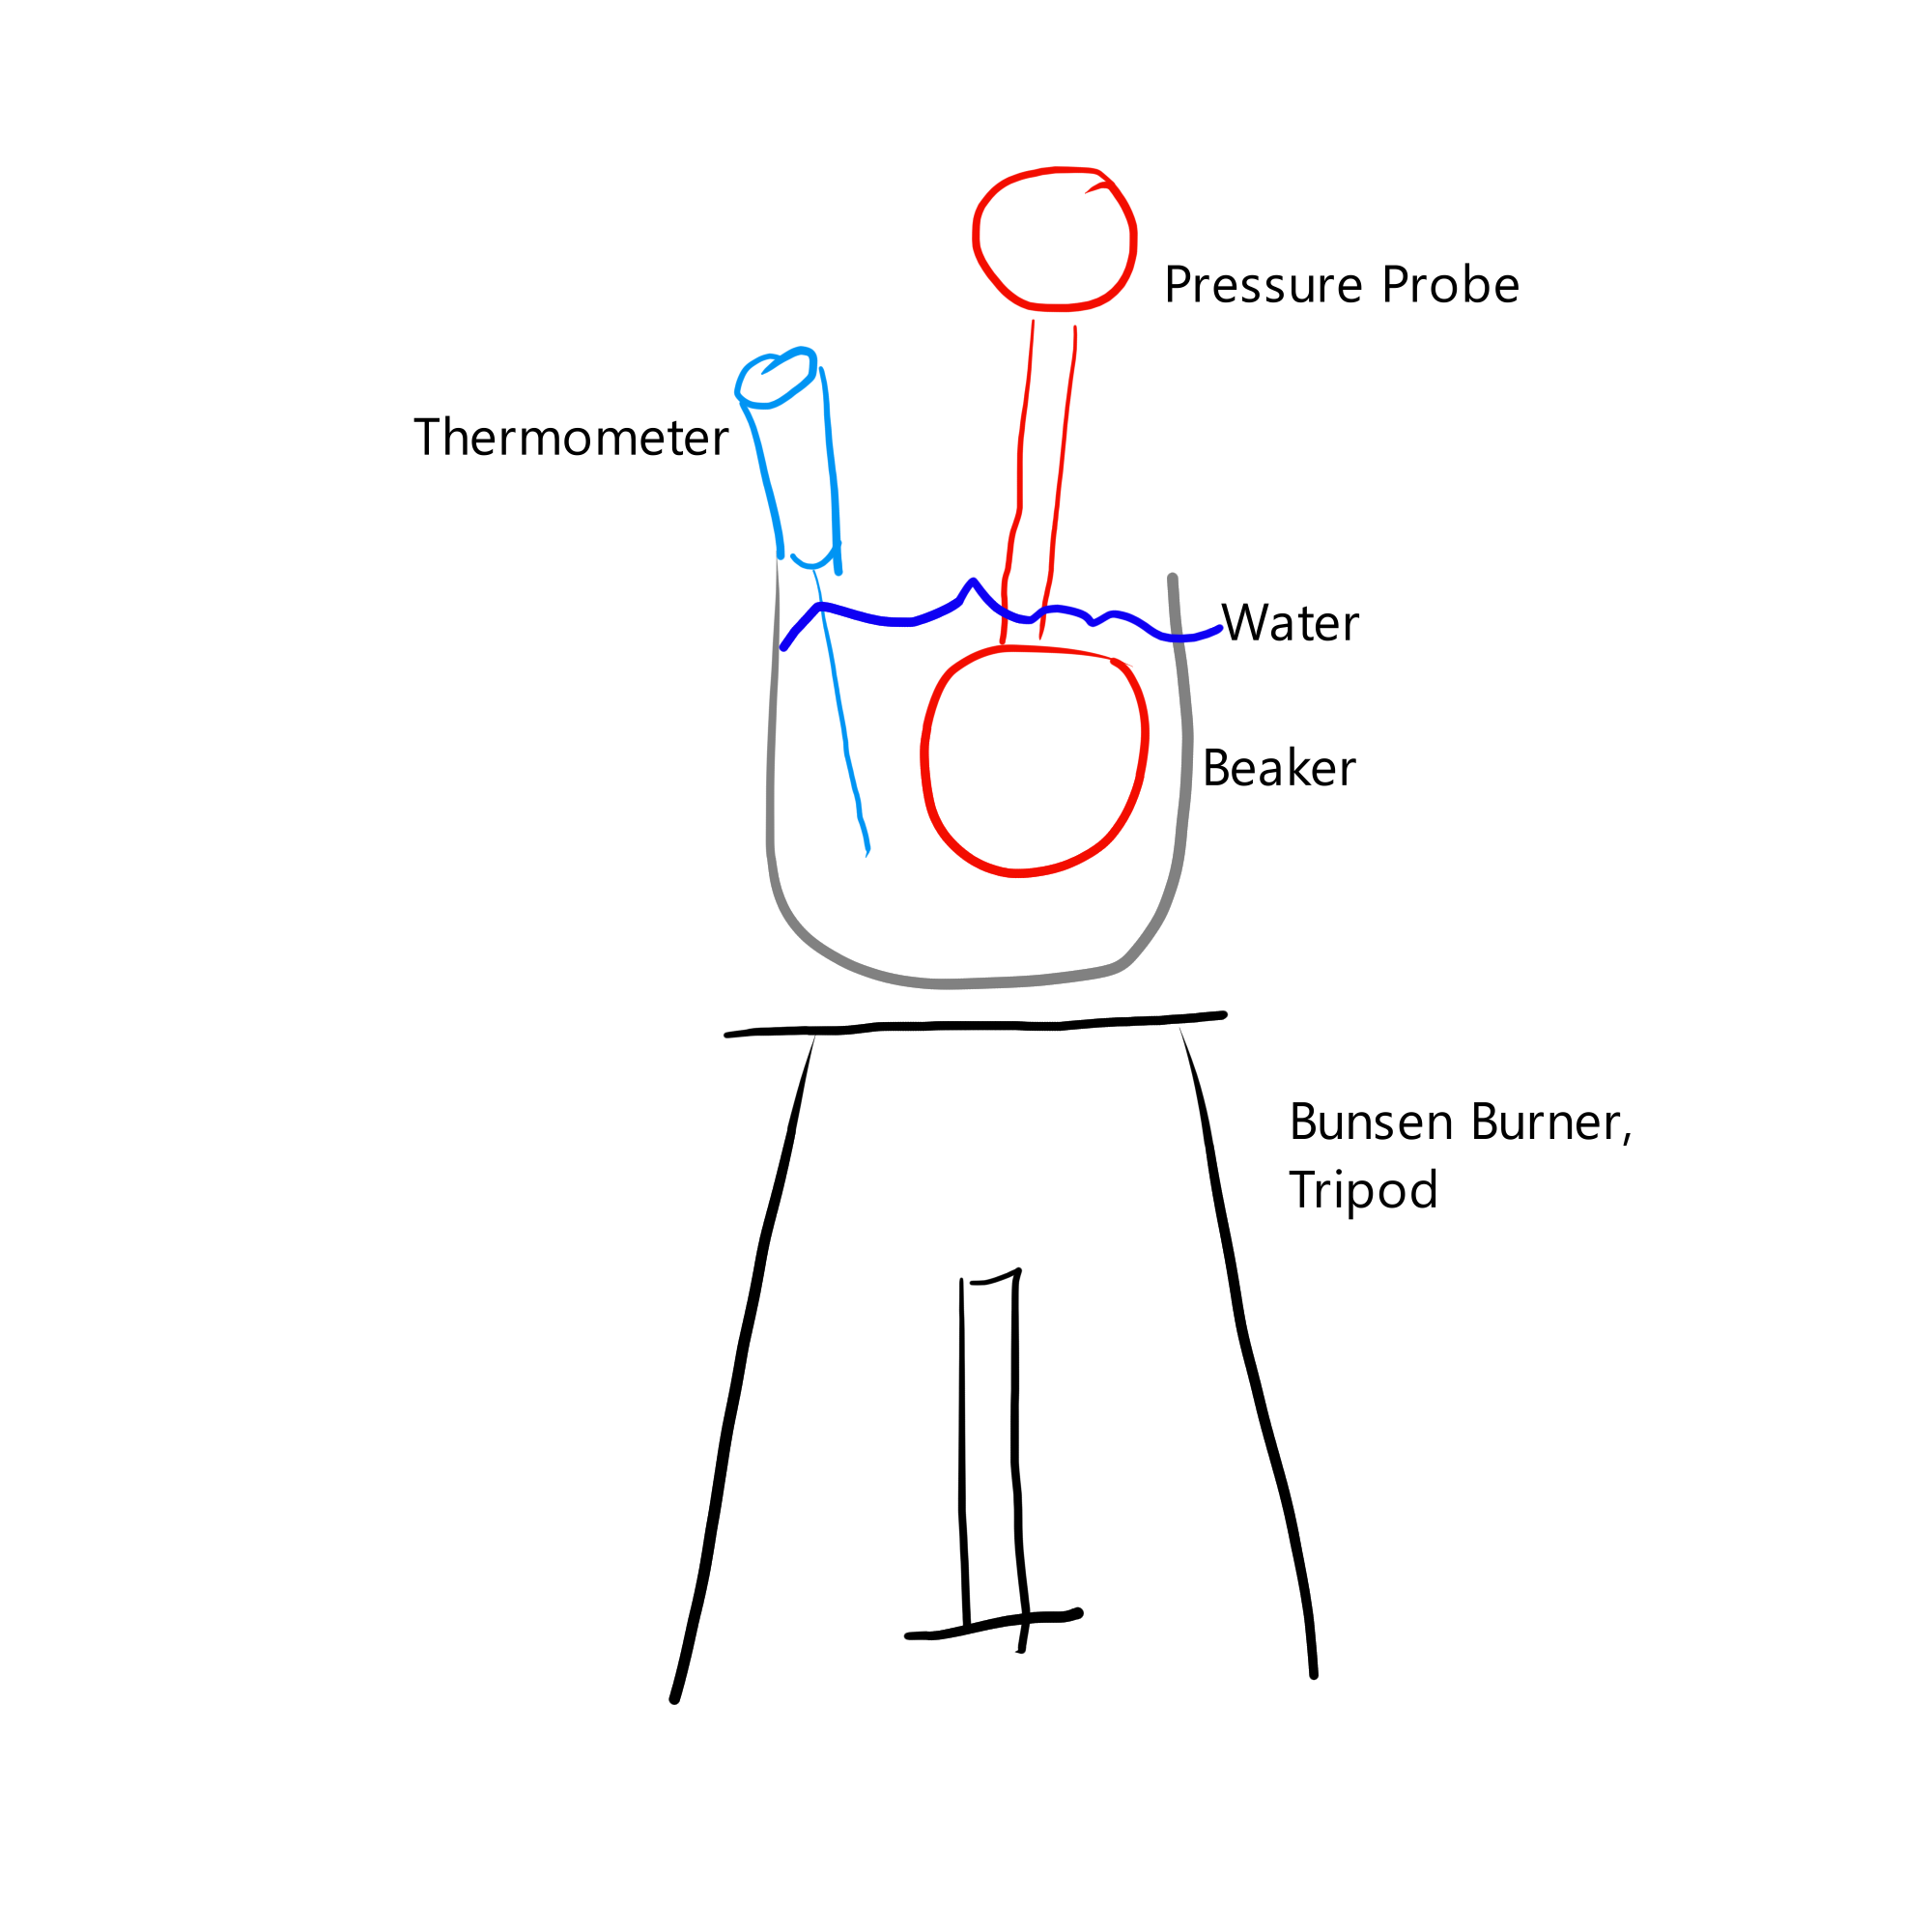
\includegraphics[scale=0.55]{assets/setupdrawn.png}
        \captionof{figure}{Drawing of the experiment setup}
        \label{fig:setupdrawn}
    \end{minipage}
\end{figure}

\subsection{Safety}
Working with pressure and high temperature presents a safety concern, wear eye protection throughout the experiment to protect against explosions.

Glass equipments are unstable during large temperature changes, care is needed in handling fragile glasswear, wear close-toe shoes and inspect the glass during the experiment and between trials to protect against accidental spills.

Take care in disposing hot water, for it can cause burns. Use a secondary beaker with cold water and slowing mix it with the primary beaker to cool it down.

\section{Data}
\subsection{Raw Data}
\subsubsection*{Qualitative data}
The endpoint of the heating is determined by the boiling of the water. In few trials, the intense boiling of the water started to shake the retort stands with the probes, causing me to end the experiment early in fear of shaking resonating, causing spilling.

The reason for a backup thermometer is because the high temperature of the water steamed up the display of the digital thermometer. I supposed operating with clamps at a dangerously high temperature is a potential safety hazard, therefore I stopped one of the trials from reach temperatures higher than 70$\si{\celsius}$.

\begin{figure}[H]
    \centering
    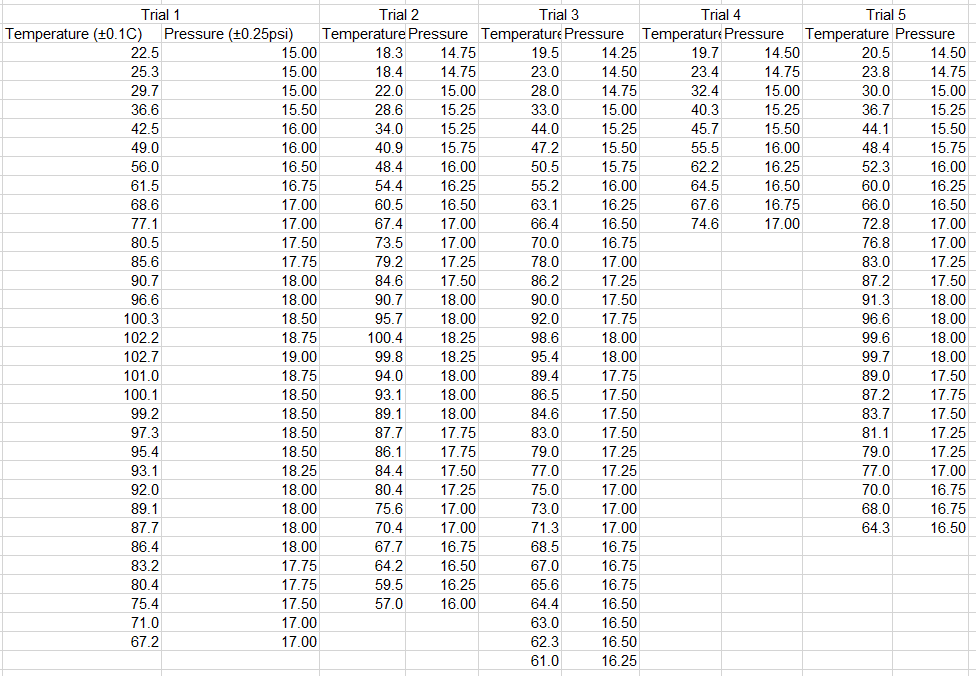
\includegraphics[width=\textwidth]{assets/rawdata.png}
    \captionof{table}{Raw quantitiative data showing the relationship between pressure and temperature}
\end{figure}

\subsection{Processing}
To convert between unit psi to kPa, the following conversion equation is used on all pressure measurements \parencite{conver_units}:
\[
    P_{\text{kPa}} \approx 6.89476 \times P_{\text{psi}}.
\]

\textit{Uncertainties}: $\relun P_{\text{kPa}} = \relun P_{\text{psi}}$

For example, in trial 1, temperature 22.5$\si{\celsius}$:

Pressure in kPa = 0.894757 $\times$ 15.00 $\approx$ $\num{1.034e+2}$,

$\absun P_{\text{psi}} = 0.25\si{psi}$

$\relun P_{\text{psi}} = \relun P_{\text{kPa}} =  \frac{0.25}{15.00} \approx 0.00667$

$\absun P_{\text{kPa}} = 0.00667 \times \num{1.034e+2} \approx \num{6.895e-1} \si{kPa}$

Therefore: $P_{\text{kPa}} = \num{1.034e+2} \pm \num{6.895e-1} \si{kPa}$


Processed data tables are in the appendix: (table \ref{fig:pq}, table \ref{fig:upq}).

\subsection{Presentation}

Transpose the pressure and temperature columns, the graph for trial 1 is shown in figure \ref{fig:t1} --- the remaining graphs for the 5 trials are in the appendix.

\begin{figure}[H]
    \centering
    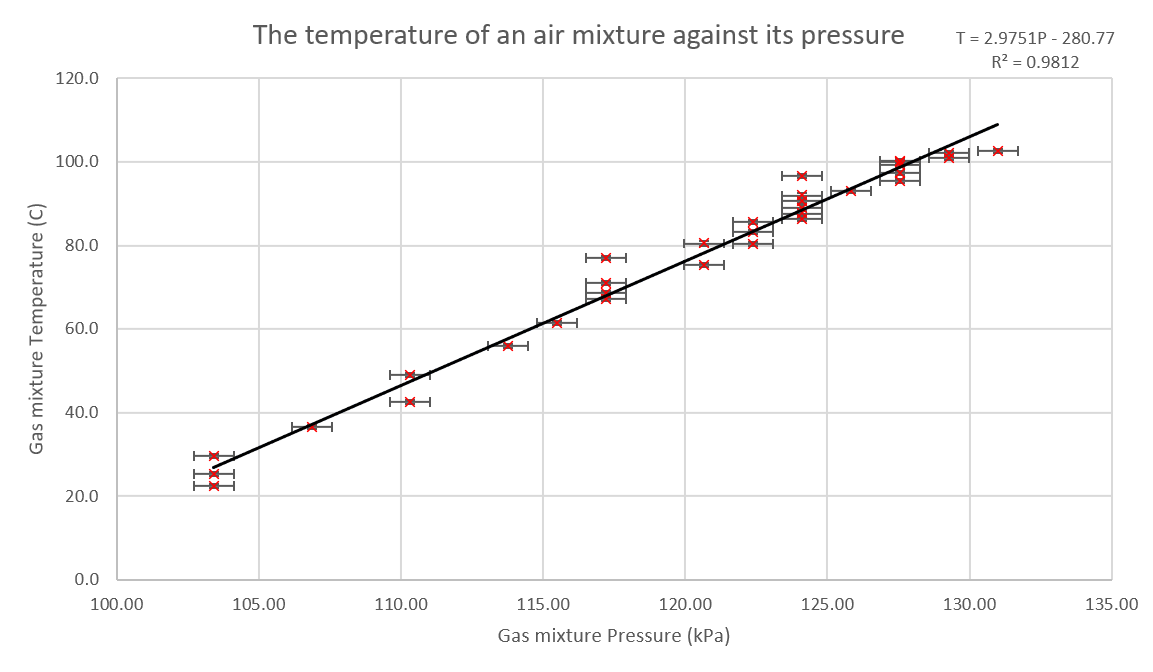
\includegraphics[width=\textwidth]{assets/graph1.png}
    \caption{Data graph for trial 1}
    \label{fig:t1}
\end{figure}

The Y error bars shows the absolute uncertainty in the thermometer, with inclusion of my reaction time. The X error bars plots the calculated absolute uncertainty of the pressure probe.

The value of absolute zero for each trial is reflected in the y-intercept of their regression line. Averaging and calculating the half range for the 5 trials will increase the accuracy of the result (figure \ref{fig:yi}).

\begin{figure}[H]
    \centering
    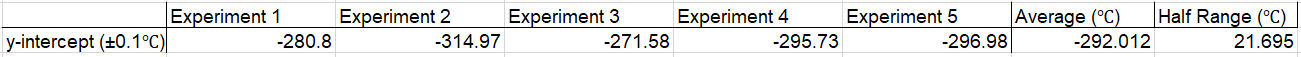
\includegraphics[scale=0.7]{assets/azerodata.png}
    \captionof{table}{The y-intercepts of the trials}
    \label{fig:yi}
\end{figure}


Mean of the y-intercepts of the trials: $\frac{\sum \text{y-intercepts}}{5} \approx -292.0 \si{\celsius}$

Half range of the y-intercepts: $\frac{\max - \min}{2} \approx 21.70 \si{\celsius}$

Therefore, our empirical value for absolute zero is: $-290 \pm 20 \si{\celsius}$

The International System of Units defines the absolute zero at $-273.15\si{\celsius}$ \parencite{si_form}, which is within our uncertainty region: $-310 < -273.15 < -270$. The percentage error of the our empirical value is: $\frac{-273.15- -290}{-273.15} \approx 6.16\%$

However, I was curious and thought to use another method to compute absolute zero using the given trial datasets. By combining the data from all of the trials onto one dataset, the result can be graphed and a regression line can be fitted (figure \ref{fig:comb}). I believe that this method will result in a more realistic value and uncertainty, given that it is analogous to conduct a really long trial with multiple cooling and heating.

\begin{figure}[H]
    \centering
    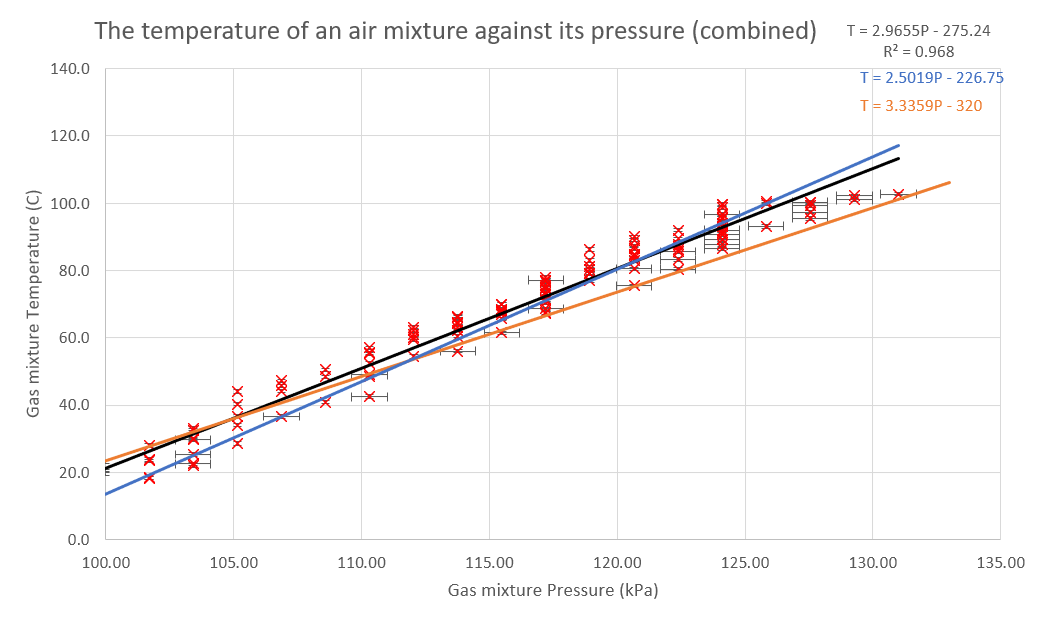
\includegraphics[width=\textwidth]{assets/combinedgraph.png}
    \caption{Data graph for the combination of datasets}
    \label{fig:comb}
\end{figure}

Using this method, the measurement of absolute zero is the value of the y-intercept of the figure. The uncertainty can be calculated using the half range between the Most Sloped line of worst fit (MSLWF) and the Least Sloped line of worst fit (LSLWF).

Y-intercept = $-275.2\si{\celsius}$

MSLWF = $-226.8\si{\celsius}$. LSLWF = $-332.0\si{\celsius}$

\textit{Uncertainty}: $\frac{\text{MSLWF} - \text{LSLWF}}{2} \approx 46.6 \si{\celsius}$

Therefore, the experimental value of absolute zero using the method is: $-270 \pm 50 \si{\celsius}$. The percentage error is: $\frac{-270 - -273.15}{-273.15} \approx 1.15\%$

\section{Conclusions}
\subsection{Result}
There exists a clear strong positive correlation between the temperature and pressure of the air mixture, as shown with the positive sloping regression line in figure \ref{fig:t1}, and the close to one correlation coefficients. This shows that as the pressure of a gas increases, the temperature will also increase, and vice versa.

% uncertainty
In both methods, there are some rather largely sized error bars in the pressure measurements. This is very likely to be caused by the rather large uncertainties of the pressure probe, for its scales have large gaps. This contributed to decreasing the precision of the value of absolute zero.
% accuracy and % error
The value and range of absolute zero computed in both methods contains the true value of absolute zero. The low percentage error of 6.16\% and 1.15\% for both methods displays the high accuracy of the data. Additionally, this suggests that the usage of multiple trials had succeeded in improving the accuracy of the outcome. The experiment data is considered to be highly accurate but lesser precise.

% theory & science involved
The high correlation coefficients in both methods showcases a strong correlation between the temperature and pressure of a gas mixture at constant volume and amount. Additionally, there were no anomalous results in the 5 trials even when the data is being collected on separate days and time. This strongly confirms my hypothesis on the relationship between gas temperature and pressure, where it is described as:
\[
    T = kP + T_{\text{absolute zero}},
\]

and $k$ is the proportionality constant. This confirms parts of the whole ideal gas law (figure \ref{fig:igl}), and showcases the validity of the kinetic theory of ideal gases.
% TODO: rephrase this more in context of the experiment
By assuming the gas mixture as an ideal gas: most important assumptions here are that the volume and intermolecular forces of particles are negligible. Because pressure is a measure of the average collision force per area of the from the particles against the container, increasing temperature increases the average kinetic energy of the particles, and increases the speed of these collision, causing higher pressure.

\subsection{Implications}
The obvious implication of the relationship between temperature and pressure is to offer a very simple procedure to measure the value of absolute zero. For past scientists, this value is the uttermost important piece of the puzzle that is in creation of the gas kinetic theory, because a non standardized unit of temperature will be plagued with minus signs at certain conditions, increasing the complexity of the formulas. This had ultimately lead to creating the field of thermodynamics.

% maybe talk about the implications of the relationship, boiling & melting points, propane gas cans and atlitudes.
% but already too much words
\subsection{Reflection}

Here is a list on the handling of the controlled variables/potential error factors, and future improvements to be made.

\subsubsection{Random Errors}
\paragraph{Large uncertainties of the pressure probe} This is very significant in contributing to the lack of precision in the dataset. The large size of the steps (0.25$\si{psi}$) in the scales and the small range of changes in the pressure relative to the scale means that a sizable temperature change may not cause a visible pressure change, leading me to note down the same value twice or more, thus increasing the spread of the data points. I have attempted to counteract this by using a timer and a constant interval, but a more precise measurement is required, I suggest to increase the range of pressure measurements --- starting with cold water instead of at room temperature, and to use a less uncertain instrument.

\paragraph{Malfunctions of the thermometer readings}
Not significant in reducing precision of temperature readings at high level, for it is controlled using a backup. The digital thermometer used does not respond nicely to heat and all the LEDs were faintly active at high temperature. If two thermometers are unavailable, consider conducting the experiment at relatively lower light levels to ease the temperature readings; or to create a plastic shield placed under the head of the thermometer.

\paragraph{Delay in data readings}
Slightly significant in increasing the spread of the dataset. The separate recording of the two sensors means that there is a random variable of delay between the temperature and pressure readings. Consider using a datalogger instead of human judgment.

\subsubsection{Systematic Errors}
\paragraph{Boiling of the water}
Relating to the controlled variable of the volume of water in the beaker, a fear of mine is that the boiling of the water will systematically shift the pressure measurements at higher temperatures upwards. The vaporization of water creates water vapor with temperature higher than $100\si{\celsius}$, heating the stem of the pressure probe and causing a systematic difference in the temperature of the air mixture and water. This is like to explain the dip in the transposed Temperature/Pressure graph in figure \ref{fig:comb}. Consider stopping the heating process at around $90-95\si{\celsius}$ to increase the accuracy of the result.

\paragraph{Environmental temperatures}
Less significant in decreasing the accuracy of the result. For the stem of the pressure probe is not submerged in to the water, a colder room temperature will systematically increase the water and air mixture temperature difference, particularly at lower temperatures. But the variable controlled in the experiment and no significant systematic shifts at lower temperatures are seen.

\paragraph{Delay in heat transfer}
The method relies on the conduction heat transfer between the water to the air mixture across glass. A systematic temperature difference in temperature may decrease the accuracy of the data points throughout all temperatures, but the low \% error indicates a low significance of this error.

\paragraph{Sensors}
In few trials, the temperature readings as the water boils is seen to increase above $100\si{\celsius}$. This showcases the systematic error of the thermometer, which shifts all points upwards in the transposed graph, resulting in a higher point of absolute zero. However, this is not the case in the experiment, which can be explained through the likely influence of the dipped higher pressure points, overwriting the systematic errors of the temperature sensor. Consider using an additional mercury thermometer alone side the digit one, and average their measurements to increase the accuracy of the final result of absolute zero.

\nocite{*}
\printbibliography


\newpage
\section*{Appendix}
\appendix
\begin{figure}[H]
    \centering
    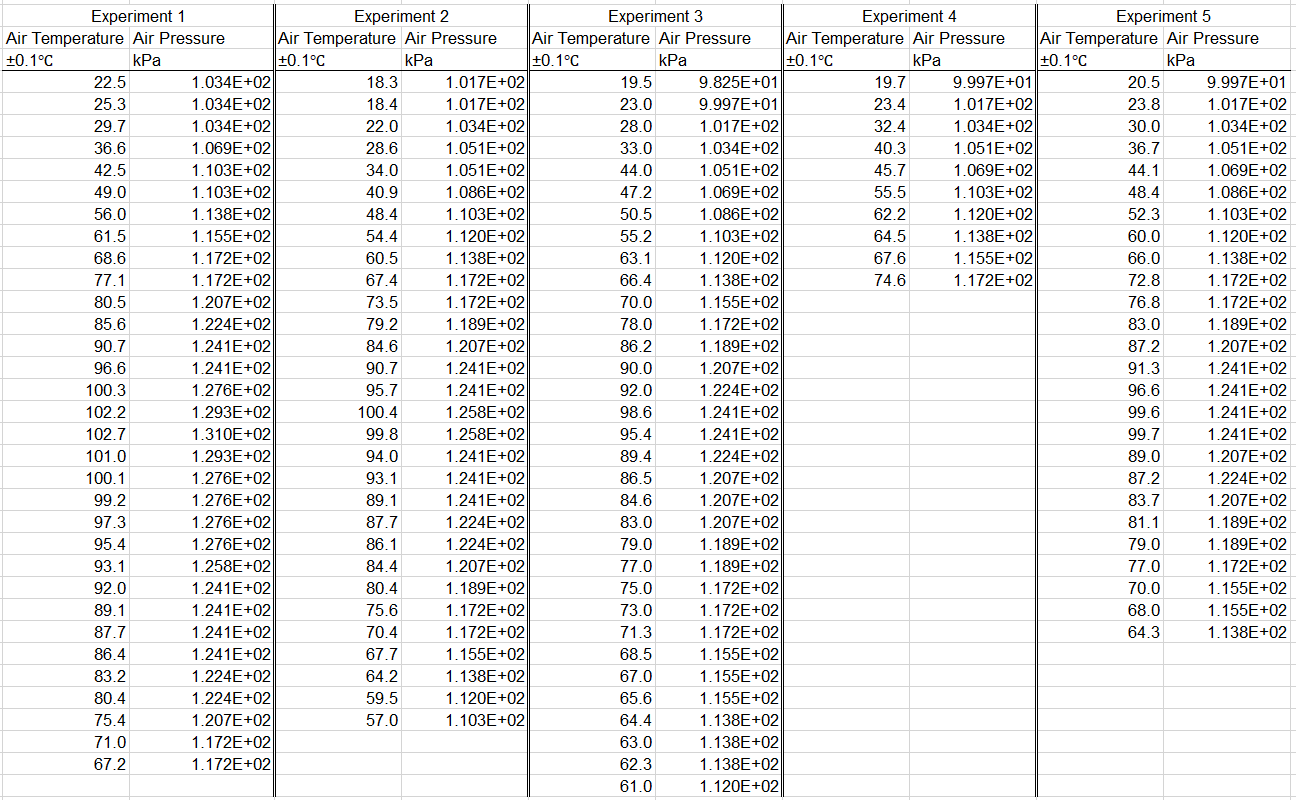
\includegraphics[scale=0.55]{assets/unitdata.png}
    \captionof{table}{Processed quantitivative data with pressure in kPa}
    \label{fig:pq}
\end{figure}

\begin{figure}[H]
    \centering
    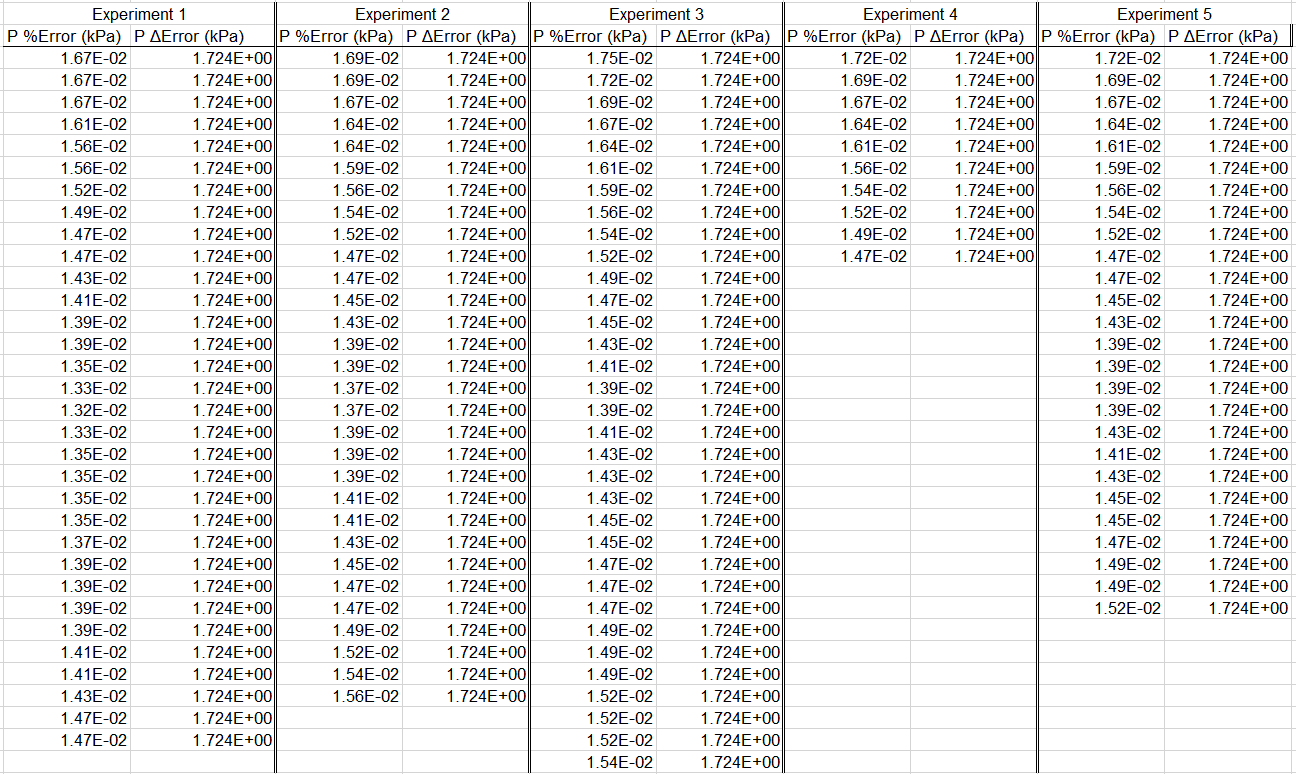
\includegraphics[scale=0.55]{assets/unitdata_unc.png}
    \captionof{table}{Uncertainty of processed quantitivative data with pressure in kPa}
    \label{fig:upq}
\end{figure}


\begin{figure}[H]
    \centering
    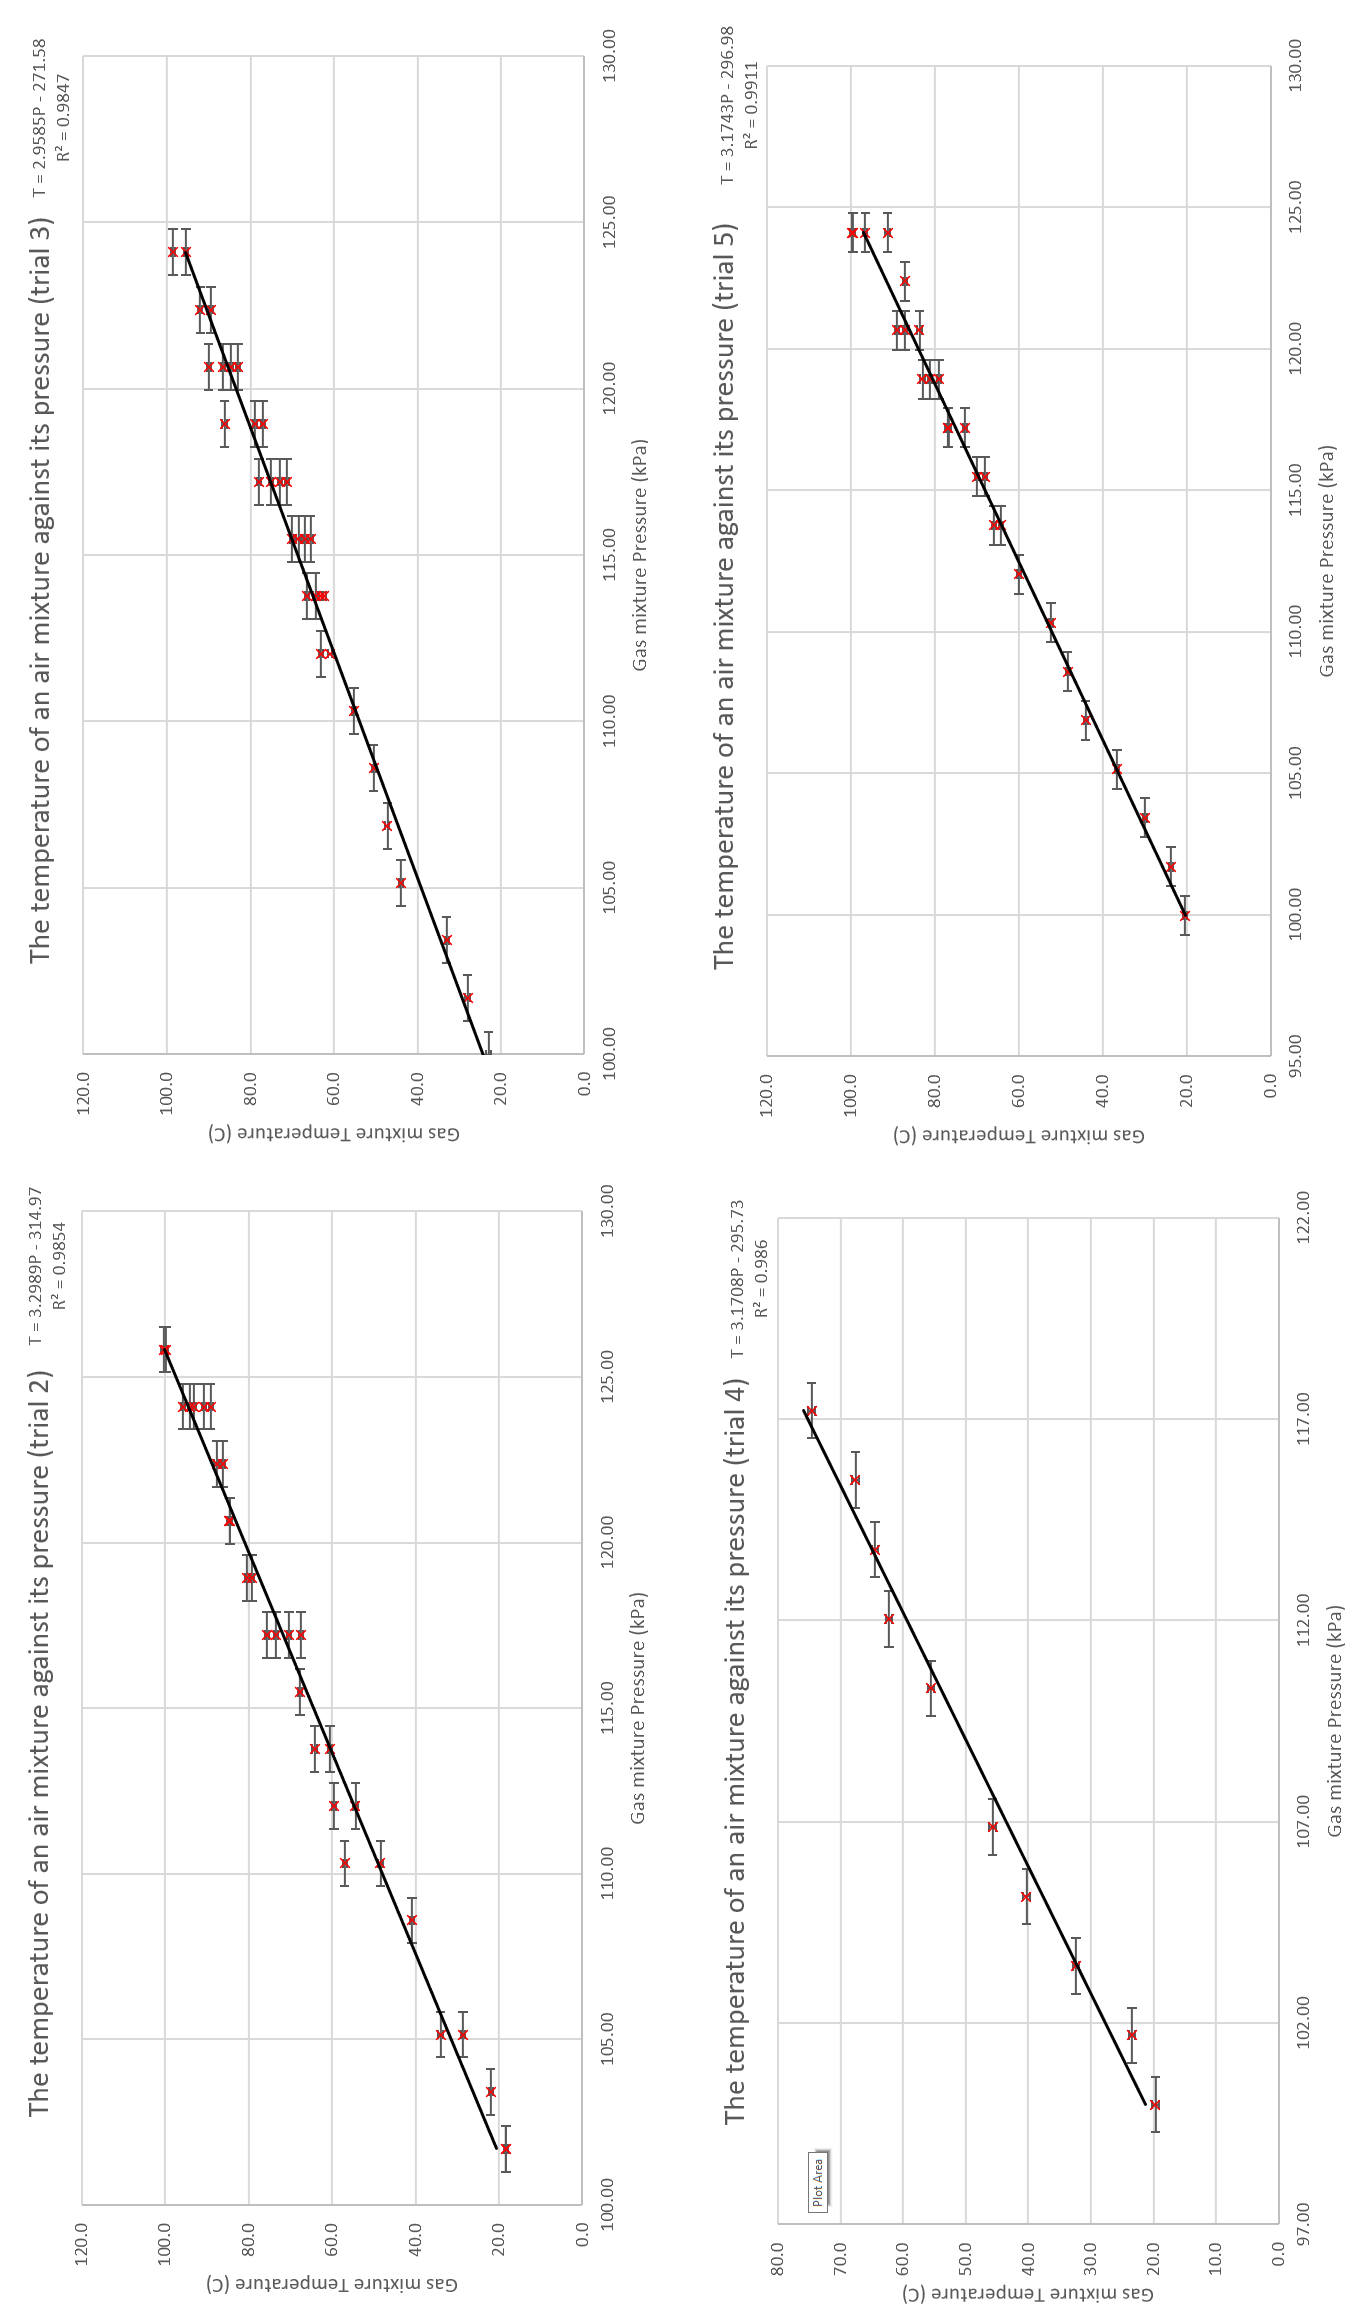
\includegraphics[width=0.87\textwidth]{assets/graphs.png}
    \captionof{figure}{Data graphs of trials 2-5}
    \label{fig:dg25}
\end{figure}

\end{document}
